\documentclass[12pt, letterpaper]{article}

%-----------------------------------------
% Frame du document
%-----------------------------------------
\usepackage[margin=2.5cm]{geometry}  % Définit les dimensions des marges
\usepackage{amsmath, amssymb}
\usepackage[french]{babel}
\usepackage[utf8]{inputenc}
\usepackage[T1]{fontenc}
\usepackage{helvet}

%-----------------------------------------
% Core
%-----------------------------------------
\usepackage{fancyhdr}           % Numérotation des pages, headers
\fancyhf{}
\usepackage{hyperref}           % Références hypertexte
\usepackage{booktabs,multirow,hhline}        % Tableaux
\usepackage{graphicx}           % Figures
\usepackage{subfig,wrapfig,caption}        % Sous-figures, ancrées, mise en forme des captions
\usepackage{titlesec}            % Mise en forme des sections
\usepackage{enumitem}           % Personnaliser les énumérations
\usepackage{color}            % Texte de couleur
\usepackage[dvipsnames]{xcolor}         % Plus de couleurs funky
\usepackage{textcomp}
\usepackage{lastpage}

%-----------------------------------------
% Math
%-----------------------------------------
\usepackage{amsmath,amssymb,amsthm,nicefrac}      % Symboles et versatilité mathématique
\usepackage{mathrsfs}           % ¯\_(ツ)_/¯ Polices d'écriture en math
\usepackage{wasysym,marvosym}         % Autres symboles math
\usepackage{mathtools}           % Peaufine la configuration des équations (when used)
\usepackage{dsfont}

%-----------------------------------------
% Physique
%-----------------------------------------
\usepackage{tikz}            % Dessine des figures
%\usepackage[american]{circuitikz}         % Dessine des schémas de circuits électroniques
\usetikzlibrary{quantikz}

\usepackage{verbatim}           % Je l'utilise pour écrire en verbatim et pour les commentaires
%\usepackage{minted}           % Ajoute du langage de prog élégamment
\usepackage{lipsum}            % Génère le lorem ispum
\usepackage{siunitx}            % Unités du système international avec \si
\usepackage{cancel}
\usepackage{todonotes}
\usepackage{empheq}
\usepackage{physics}
% \usepackage{bm}% Your new best friend in LaTeX
% http://ctan.math.ca/tex-archive/macros/latex/contrib/physics/physics.pdf      La documentation dudit merveilleux package

\usepackage{float}

\usepackage{halloweenmath} % décorations d'halloween pour vos devoirs (J'encourage l'utilisation de la sorcière mathémagique avec \mathwitch )

\def\CQFD{\begin{flushright}CQFD.\end{flushright}}
\def\RANCHITUP{\begin{flushright}CQFD.\end{flushright}}
\def\PIFPAF{\begin{flushright}CQFD.\end{flushright}}
% \RANCHITUP ou \PIFPAF pour écrire un CQFD bien placé

\newcommand{\uvec}[1]{\boldsymbol{\hat{\textbf{#1}}}}
\newcommand{\uveci}{{\bm{\hat{\textnormal{\bfseries\i}}}}}
\newcommand{\uvecj}{{\bm{\hat{\textnormal{\bfseries\j}}}}}
% Beaux vecteurs unitaires avec \uvec


\newcommand{\del}[2]{\frac{\partial #1}{\partial #2}}
\newcommand{\delp}[1]{\frac{\partial }{\partial #1}}
\newcommand{\ddfrac}[2]{\frac{\dd #1}{\dd #2}}
\newcommand{\ddfracp}[1]{\frac{\dd }{\dd #1}}
\newcommand{\braAket}[3]{\left<#1\left|#2\right|#3\right>}


%-----------------------------------------
% Références
%-----------------------------------------
\numberwithin{table}{section}
\numberwithin{figure}{section}
\numberwithin{equation}{section}


\begin{document}

\title{Devoir 4 : Simulation Monte Carlo du modèle de Ising}
\author{PHQ404}
\date{Date de complétion suggérée: 5 avril 2024 à 23h45}
\maketitle

\section{Objectif}\label{sec:objectif}

\noindent L'objectif de ce devoir est d'étudier une transition de phase
dans le modèle de Ising en 2 dimensions.


\section{Comment présenter et remettre votre TP}\label{sec:comment-presenter-et-remettre-votre-tp}

\noindent Vous devez cloner le répertoire github dans l'organisation du cours au lien suivant :\\
\href{https://classroom.github.com/a/dDkgRxSQ}{https://classroom.github.com/a/dDkgRxSQ}.
Dans ce répertoire se trouvera votre code python, vos tests unitaires ainsi que votre rapport
décrivant les méthodes utilisés et l'analyse de vos résultats.
La structure des fichiers ne doit pas être modifiée, mais vous pouvez ajouter des fichiers si vous le désirez.
Voici la structure de fichiers que votre répertoire devra garder :

\bigskip

Root
\begin{itemize}
    \item[]
        \begin{itemize}
            \item[$\rightarrow$] src
                \begin{itemize}
                    \item[$\hookrightarrow$] \texttt{fichier0.py}
                    \item[$\hookrightarrow$] \texttt{fichier1.py}
                    \item[$\hookrightarrow$] \dots
              \end{itemize}
        \end{itemize}
  \item[]
  \begin{itemize}
    \item[$\rightarrow$] tests
    \begin{itemize}
      \item[$\hookrightarrow$] \texttt{test\_fichier0.py}
      \item[$\hookrightarrow$] \texttt{test\_fichier1.py}
      \item[$\hookrightarrow$] \dots
    \end{itemize}
  \end{itemize}
  \item[$\hookrightarrow$] \texttt{.gitignore}
  \item[$\hookrightarrow$] \texttt{requirements.txt}
  \item[$\hookrightarrow$] \texttt{README.md}
\end{itemize}

\bigskip

\noindent Le fichier \texttt{requirements.txt} doit contenir les dépendances de votre projet.
Le fichier \\\texttt{README.md} doit contenir les instructions pour installer et utiliser votre projet ainsi
qu'une brève description du devoir et des méthodes utilisés dans le code.
Voir la section~\ref{sec:Readme} pour plus de détails.
Dans le dossier \texttt{src} se trouvera votre code python et dans le dossier \texttt{tests} se trouvera vos tests
unitaires.

\bigskip

\noindent La remise et la correction automatique du code se fera à chaque \texttt{push} sur le répertoire github.
Notez que seul le dernier \texttt{push} sur la branche \texttt{main} sera considéré pour la correction.


\section{Énoncé}\label{sec:enonce}

\subsection{Modèle de Ising}\label{subsec:modele-de-ising}

\noindent Un fichier python est joint à ce devoir.
Celui-ci contient une classe nommée \textit{Ising} qui permet de représenter
un système de spins ferromagnétique avec un couplage entre les premiers voisins.
La classe est cependant incomplète et vous devez compléter l'implémentation
de certaines méthodes.
Pour ce faire, vous pouvez ajouter des méthodes intermédiaires,
mais vous ne pouvez pas retirer de méthodes.

\bigskip

\noindent La classe est compilée avec la bibliothèque \textit{NumBa} pour accélérer les calculs.
Cependant, cela impose des contraintes sur les versions de \textit{NumPy}.
En effet, il est important de choisir une version de numpy avant 1.22 pour éviter des problèmes
de compatibilité.

\subsection{Méthode du binning}\label{subsec:methode-du-binning}

\noindent Une seconde classe nommée \textit{Observable} est également fournise pour
évaluer des statistiques sur l'aimantation et l'énergie à l'aide de la méthode du binning.
Vous devez également compléter cette classe.

\subsection{Simulation Monte Carlo}\label{subsec:simulation-monte-carlo}

\noindent À l'aide de ces deux classes, vous devez implémenter une simulation Monte Carlo
pour un système de $32 \times 32$ spins pour des températures entre $1.0$ et $4.0$
par incrément de $0.1$.
Pour ce faire, vous devez
\begin{enumerate}
    \item initialiser le système aléatoirement;
    \item effectuer 1 000 000 d'itérations pour réchauffer le système;
    \item rendre une mesure de l'énergie et de l'aimantation après chaque interval de 1 000 itérations;
    \item terminer la simulation après avoir accumuler $2^{16}$ mesures;
    \item enregistrer les résultats dans un fichier de données.
\end{enumerate}

\subsection{Visualisation des résultats}\label{subsec:visualisation-des-resultats}

\noindent Vous devez fournir des graphiques similaires aux figures suivantes
et commenter brièvement les résultats.
Attention, ne vous fiez pas au format des graphiques puisqu'ils ne sont pas dignes d'un rapport scientifique.

\begin{figure}[H]
    \begin{center}
        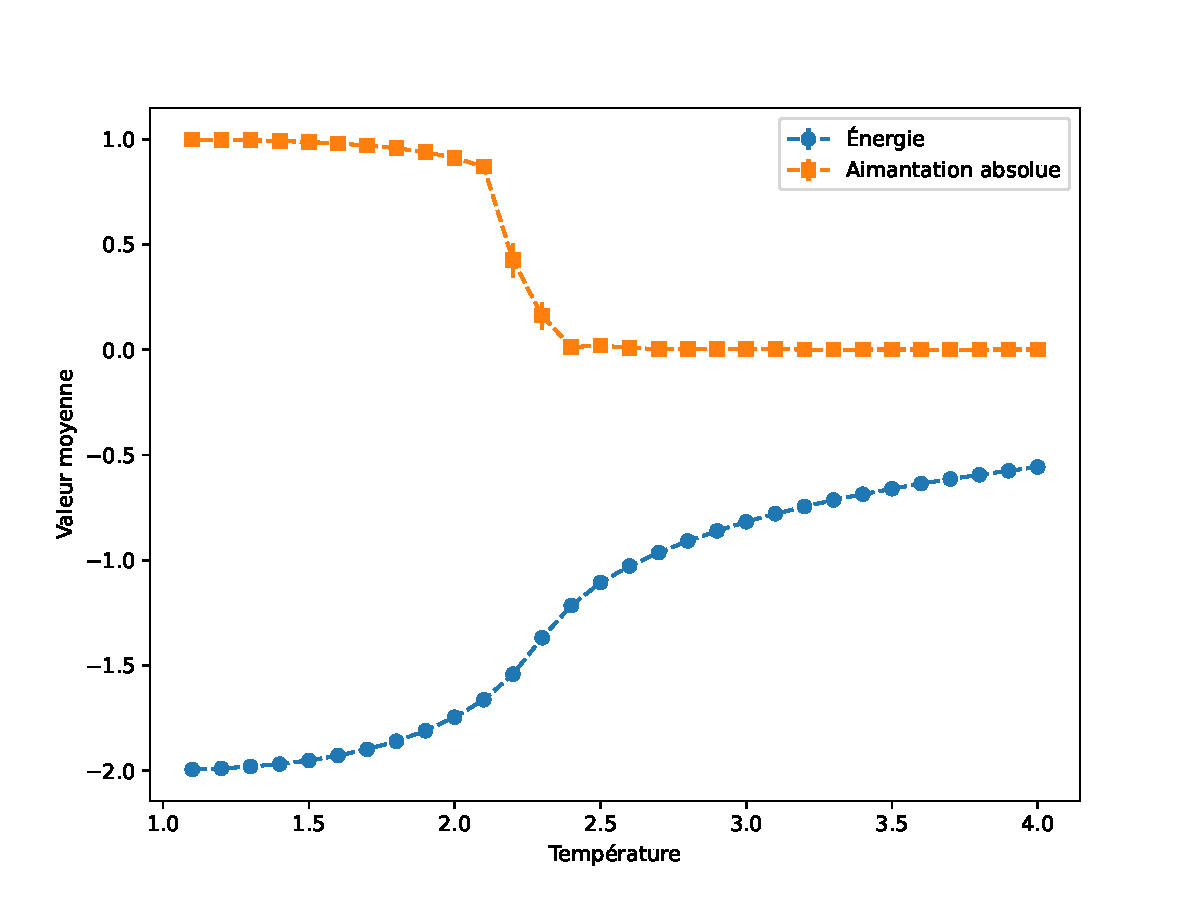
\includegraphics[width=0.75\textwidth]{../images/energie_aimantation}
    \end{center}
    \caption{
        Exemple de figure pour les valeurs moyennes et les erreurs d'estimation
        pour l'énergie et l'aimantation par spin selon la température.
        Les erreurs d'estimation sont obtenues avec la méthode du binning de 16 niveaux.
    }
    \label{fig:moyennes}
\end{figure}

\begin{figure}[H]
    \begin{center}
        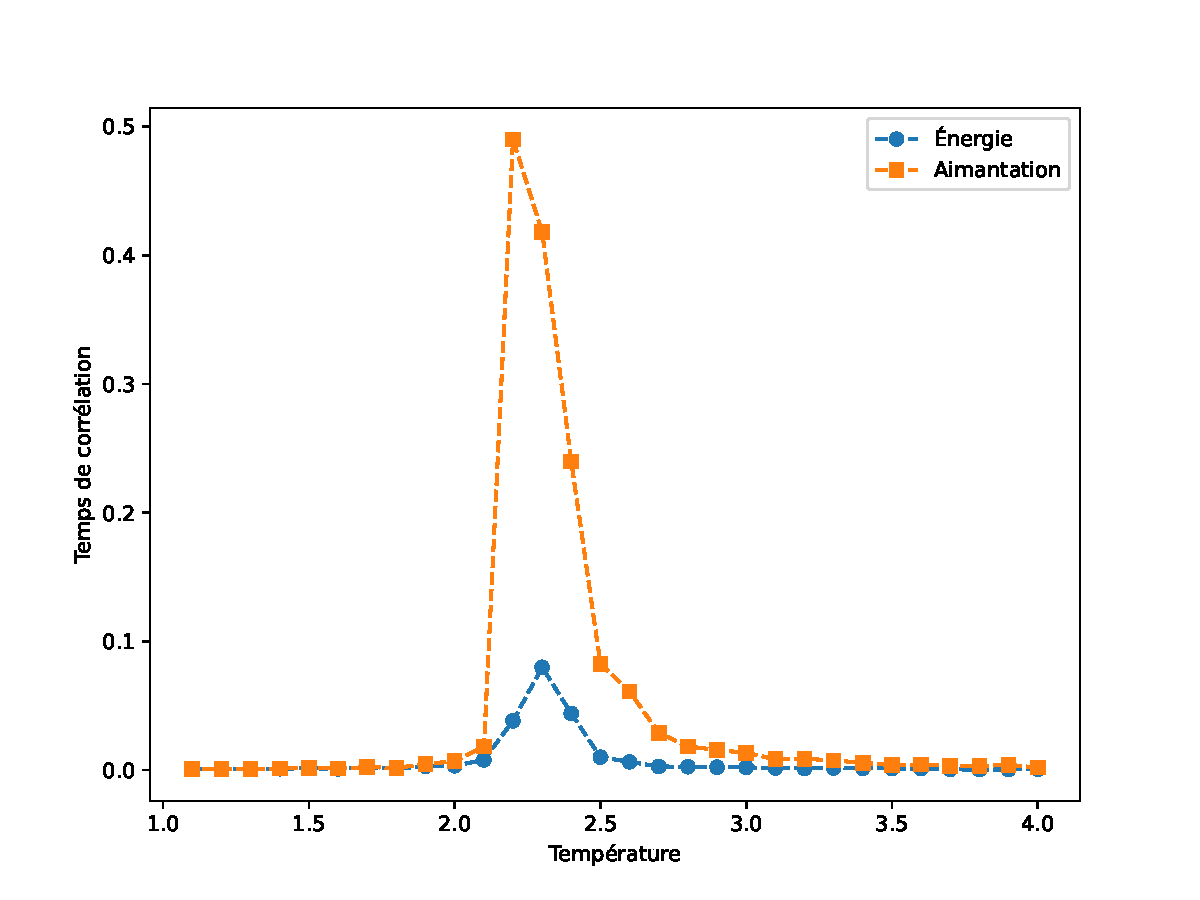
\includegraphics[width=0.75\textwidth]{../images/temps_correlation}
    \end{center}
    \caption{
        Exemple de figure pour les temps de corrélation selon la température.
    }
    \label{fig:correlation}
\end{figure}

\bigskip

\noindent Note: Toutes les fonctions qui doivent être implémentées sont déjà définies dans les fichiers
et retournent des \texttt{NotImplementedError}.


\section{Vérification}\label{sec:verification}

\noindent Il est important de vérifer vos implémentations.
En effet, vous devez vous assurer que vos méthodes fonctionnent correctement et pour ce faire, vous devez rouler et
implémenter des tests unitaires qui testent chacune de vos classes et fonctions.
De plus, vous devriez tester si les résultats obtenus sont logiques.
Il serait aussi intéressant de retrouver vos vérifications dans votre rapport.
Il est fortement recommandé d'ajouter des tests unitaires dans le dossier \texttt{tests}, mais les tests déjà
implémentés ne doivent pas être modifiés.


\section{Readme}\label{sec:Readme}

\noindent Vous devez faire un fichier Readme qui explique ce que contient votre répertoire et comment l'utiliser.
Le Readme sera divisé en 2 parties: une partie plus courte qui consiste essentiellement à ce qu'on retrouve normalement
dans Readme scientifique et une partie plus longue qui consiste en une présentation et analyse des résultats.

\bigskip

\noindent La première partie doit contenir les éléments suivants:
\begin{itemize}
    \item Une brève description du contenue du répertoire;
    \item Une figure qui résume le contenu du répertoire ainsi que les résultats principaux;
    \item Les instructions pour installer et utiliser votre projet.
\end{itemize}
Il faut qu'un utilisateur externe soit en mesure de regarder la première partie du Readme et comprendre en quelques
secondes le contenu du répertoire, les résultats principaux et comment utiliser le projet.
C'est important d'être concis, clair et efficace.
Pour la figure, il sagit d'une image permettant au lecteur de comprendre rapidement le contenu du répertoire.
Celle-ci pourrait être, par exemple, un diagramme représentant le pipeline de traitement des données, un graphique
comparant les différentes méthodes implémentées, etc.

\bigskip

\noindent Le deuxième partie doit contenir les éléments suivants:
\begin{itemize}
    \item Une plus longue description du contenu du répertoire;
    \item Une présentation et explication des méthodes utilisées;
    \item Une présentation des résultats obtenus;
    \item Une analyse des résultats obtenus;
    \item Une conclusion.
\end{itemize}
Cette seconde partie sert à expliquer en quoi consiste ce dépôt si l'utilisateur décidait que la première partie
du Readme était assez intéressante et bien présentée pour qu'il veuille en savoir plus.
Il sagit ici d'un court rapport scientifique.
Il faut donc rester concis afin d'être lu en quelques minutes seulement, mais mettre suffisamment d'information pour
que l'utilisateur comprenne bien la théorie, les méthodes et les résultats.



\section{Critères d'évaluation}\label{sec:criteres-d'evaluation}

\begin{description}
  \item[70 points] Pour le résultat de l'autocorrection du code obtenue à l'aide du module TAC\@.
  \item[30 points] Pour la qualité du Readme.
\end{description}


\end{document}
